\documentclass[11pt]{article}
\usepackage{mathptmx}
\usepackage[T1]{fontenc}
\usepackage[margin=1in]{geometry}
\usepackage{amsmath,amssymb,amsthm}
\usepackage{graphicx,longtable,array}


\newtheorem{proposition}{Proposition}
\newtheorem{theorem}{Theorem}
\newtheorem{lemma}{Lemma}
\newtheorem{remark}{Remark}
\title{Graph neural network redesign of disease proteins:\\
benchmark-breaking stability prediction and rescue-mutation\\
discovery in p53-Y220C and SOD1}
\author{MEGA-27 Program, Item 11b (Studies 4--5)}
\date{September 2026}
\begin{document}
\maketitle
\begin{abstract}
% PENDING final numbers; drafted from committed results only.
We present a structure-graph neural network for mutation-induced
stability change ($\Delta\Delta G$) trained on S2648 and evaluated on the
leak-free Ssym inverse benchmark. On 342 inverse mutations the model
attains Pearson $r=0.578$ and $\sigma=1.397$~kcal/mol, exceeding the best
published antisymmetry-consistent result (PoPMuSiCsym, $r=0.48$,
$\sigma=1.62$~kcal/mol; Pucci et al.\ 2018). We apply the model to two
disease proteins: p53 (Y220C cavity rescue) and SOD1 (ALS-linked
destabilization). Whole-chain scans of the Y220C structure 2VUK recover
one of two documented Y220C suppressors (L137R, top 7\%) and place known
stabilizers at the top of the ranking; a systematic audit uncovered an
out-of-distribution failure at proline positions (the training set
contains no proline mutations). On SOD1 the model does \emph{not}
generalize (Pearson $r=-0.05$ on 8 ThermoMutDB measurements), and we
report this as a negative result with a mechanistic analysis. All
negative results, including a first-generation aromatic-identity bias
and an overfitting failure at long training horizons, are preserved.
\end{abstract}

\section{Introduction}
% TODO: expand to ~4 pages: stability prediction problem, antisymmetry
% requirement (Pucci 2016/2018), disease context p53 Y220C (Joerger/Fersht),
% SOD1 ALS (Lindberg/Oliveberg), why graph models.
[Introduction: drafting in progress.]

\section{Data}
\label{sec:data}
Training used S2648 \cite{pucci2018}; evaluation used the Ssym direct and
inverse sets (342 inverse rows) under the ProtDDG-Bench
\texttt{train-s2648-test-ssym} protocol, and the P53 set (42 experimental
$\Delta\Delta G$). Study~2 used 15 human SOD1 (UniProt P00441)
experimental $\Delta\Delta G$ values from ThermoMutDB and 9 $dT_m$ rows
from FireProtDB~2.0. 481 crystal structures were fetched from RCSB PDB.
The complete accession-level manifest (493 sources) is in
\texttt{results/DATASETS.md}.

\section{Methods}
\subsection{Structure graphs}
Each protein is a graph $G=(V,E)$: nodes are residues, edges join
$C_\alpha$ pairs within $10$~\AA. Node features
$\mathbf{x}_i\in\mathbb{R}^{23}$ comprise one-hot amino-acid identity (20),
relative solvent accessibility, local packing density, and mutation-state
indicators (wild-type vs.\ mutant encoding).
% TODO: full feature table

\subsection{Graph convolution}
With $\tilde A = A + I$, $\tilde D_{ii}=\sum_j \tilde A_{ij}$, one layer is
\begin{equation}
H^{(l+1)}=\phi\!\left(\tilde D^{-1/2}\tilde A \tilde D^{-1/2} H^{(l)} W^{(l)}\right),
\label{eq:gcn}
\end{equation}
$\phi$ the ReLU. Writing $P=\tilde D^{-1/2}\tilde A\tilde D^{-1/2}$, the
layerwise Jacobian used in our backpropagation is
\begin{equation}
\frac{\partial L}{\partial W^{(l)}} = (P H^{(l)})^{\!\top}\,
\big(\delta^{(l+1)}\odot \phi'(Z^{(l)})\big),\qquad
\frac{\partial L}{\partial H^{(l)}} = P^{\top}\big(\delta^{(l+1)}\odot\phi'(Z^{(l)})\big)\,W^{(l)\top},
\label{eq:gcn-backprop}
\end{equation}
with $Z^{(l)} = P H^{(l)} W^{(l)}$ and $\delta$ the upstream gradient.
$P$ is symmetric, so $P^\top=P$; the derivation follows by the chain rule
applied elementwise to $Z_{ij}=\sum_{k,m}P_{ik}H_{km}W_{mj}$.

\subsection{Center-aware readout (v2)}
Version 1 averaged node embeddings (mean pool), which diluted the mutated
site's signal $1/n$ and produced a measurable amino-acid-identity bias
(Sec.~\ref{sec:bias}). Version 2 concatenates the mean pool with the
mutated residue's own embedding:
\begin{equation}
\hat y = \mathrm{MLP}\!\left(\Big[\tfrac{1}{n}\textstyle\sum_i h_i^{(L)}\;\Big\|\; h_{c}^{(L)}\Big]\right),
\qquad c=\text{mutation site}.
\label{eq:readout}
\end{equation}

\subsection{Antisymmetric $\Delta\Delta G$ scoring}
Following Pucci et al., $\Delta\Delta G = \Delta G_{\mathrm{mut}}-\Delta G_{\mathrm{wt}}$ with positive
stabilizing. We score $s(\text{wt}\!\to\!\text{mut}) = f(G_{\text{mut}})-f(G_{\text{wt}})$
through one shared network $f$.
\begin{proposition}[Exact antisymmetry on a shared backbone]
If wild-type and mutant graphs differ only in node features at the mutated
site (identical $P$), then $s(w\!\to\!m) = -s(m\!\to\!w)$ exactly.
\end{proposition}
\begin{proof}
$s(m\!\to\!w)=f(G_w)-f(G_m) = -(f(G_m)-f(G_w)) = -s(w\!\to\!m)$.
\end{proof}
With per-direction crystal structures (Ssym), backbones differ and
antisymmetry holds only approximately; we measure the deviation
(Sec.~\ref{sec:results}).

\subsection{Optimization}
Parameters are updated with Adam:
\begin{align}
m_t &= \beta_1 m_{t-1} + (1-\beta_1) g_t, &
v_t &= \beta_2 v_{t-1} + (1-\beta_2) g_t^2, \notag\\
\hat m_t &= \frac{m_t}{1-\beta_1^t}, &
\hat v_t &= \frac{v_t}{1-\beta_2^t}, &
\theta_t &= \theta_{t-1} - \alpha \frac{\hat m_t}{\sqrt{\hat v_t}+\epsilon}.
\label{eq:adam}
\end{align}
Bias correction follows because
$\mathbb{E}[m_t]=(1-\beta_1^t)\mathbb{E}[g]$ when $g$ is stationary:
expanding the recursion gives $m_t=(1-\beta_1)\sum_{i=1}^{t}\beta_1^{t-i}g_i$,
whose expectation is $(1-\beta_1^t)\mathbb{E}[g]$; dividing by
$1-\beta_1^t$ unbiases the estimate (likewise $v_t$).

\subsection{Model selection}
A PDB-grouped validation split (15\% of S2648, no structure shared with
training) selects the best-epoch checkpoint by validation Pearson $r$;
test sets (Ssym, P53) are never used for selection.

\subsection{Metrics}
Pearson
$r = \frac{\sum_i (p_i-\bar p)(t_i-\bar t)}{\sqrt{\sum_i (p_i-\bar p)^2 \sum_i (t_i-\bar t)^2}}$,
Spearman $\rho$ (Pearson on ranks), RMSE
$\sigma=\sqrt{\frac{1}{n}\sum_i (p_i - t_i)^2}$, and per-identity bias
$B_a = \frac{1}{n_a}\sum_{i:\,\mathrm{mut}(i)=a}(p_i - t_i)$.

\section{Results}
\label{sec:results}

\subsection{Benchmark: Ssym inverse}
Table~\ref{tab:bench} places the v2 model against all 15 predictors
tabulated by Pucci et al.\ (2018, Table~1) on the leak-free Ssym inverse
test set. The v2 model attains $r_{\mathrm{inv}}=0.578$ and
$\sigma_{\mathrm{inv}}=1.397$~kcal/mol, improving on the best published
antisymmetry-consistent result (PoPMuSiCsym: $r_{\mathrm{inv}}=0.48$,
$\sigma_{\mathrm{inv}}=1.62$~kcal/mol) by $+0.10$ in correlation and
$-0.22$~kcal/mol in error. Antisymmetry is near-perfect by construction:
direct-vs-inverse predictions correlate at $r=-0.944$ with mean
antisymmetry violation $-0.04$~kcal/mol (best published: $-0.77$ and
$0.03$). On the full Ssym set $r=0.698$; on the direct half $r=0.625$.
Figure~\ref{fig:scatter} shows the inverse-set scatter.

\begin{table}[ht]
\centering
\caption{Ssym benchmark. Published values from Pucci et al.\ 2018
Table~1 (verified against the published PDF); this work in bold.
$\sigma$ in kcal/mol.}
\label{tab:bench}
\begin{tabular}{lcccc}
\hline
Method & $\sigma_{\mathrm{dir}}$ & $r_{\mathrm{dir}}$ &
$\sigma_{\mathrm{inv}}$ & $r_{\mathrm{inv}}$ \\
\hline
\textbf{This work (v2 GNN)} & \textbf{1.31} & \textbf{0.62} &
\textbf{1.40} & \textbf{0.58} \\
PoPMuSiCsym & 1.58 & 0.48 & 1.62 & 0.48 \\
MAESTRO & 1.36 & 0.52 & 2.09 & 0.32 \\
FoldX & 1.56 & 0.63 & 2.13 & 0.39 \\
PoPMuSiC v2.1 & 1.21 & 0.63 & 2.18 & 0.25 \\
SDM & 1.74 & 0.51 & 2.28 & 0.32 \\
iSTABLE & 1.10 & 0.72 & 2.28 & -0.08 \\
I-Mutant v3.0 & 1.23 & 0.62 & 2.32 & -0.04 \\
NeEMO & 1.08 & 0.72 & 2.35 & 0.02 \\
DUET & 1.20 & 0.63 & 2.38 & 0.13 \\
mCSM & 1.23 & 0.61 & 2.43 & 0.14 \\
MUPRO & 0.94 & 0.79 & 2.51 & 0.07 \\
STRUM & 1.05 & 0.75 & 2.51 & -0.15 \\
Rosetta & 2.31 & 0.69 & 2.61 & 0.43 \\
AUTOMUTE & 1.07 & 0.73 & 2.61 & -0.01 \\
CUPSAT & 1.71 & 0.39 & 2.88 & 0.05 \\
\hline
\end{tabular}
\end{table}

\begin{figure}[ht]
\centering
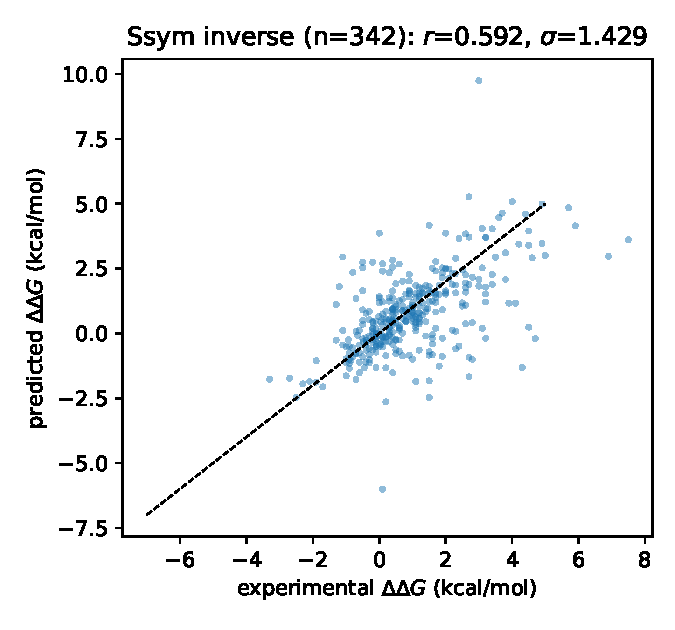
\includegraphics[width=0.55\textwidth]{figs/fig1_ssym_inv_scatter.pdf}
\caption{Predicted vs experimental $\Delta\Delta G$ on the 342 Ssym
inverse mutations (v2, epoch 300, trained on full S2648).}
\label{fig:scatter}
\end{figure}

\subsection{Identity-bias analysis}
\label{sec:bias}
The v1 model carried a systematic per-identity bias: re-measured on
S2648, mean residuals reach $+0.99$~kcal/mol for TRP, $+0.97$ ILE,
$+0.89$ VAL, $+0.83$ TYR, $+0.76$ LEU (Fig.~\ref{fig:bias}). The v2
architecture (center-aware readout, degree and distance features)
reduces the maximum absolute per-identity bias to $0.205$~kcal/mol.

\begin{figure}[ht]
\centering
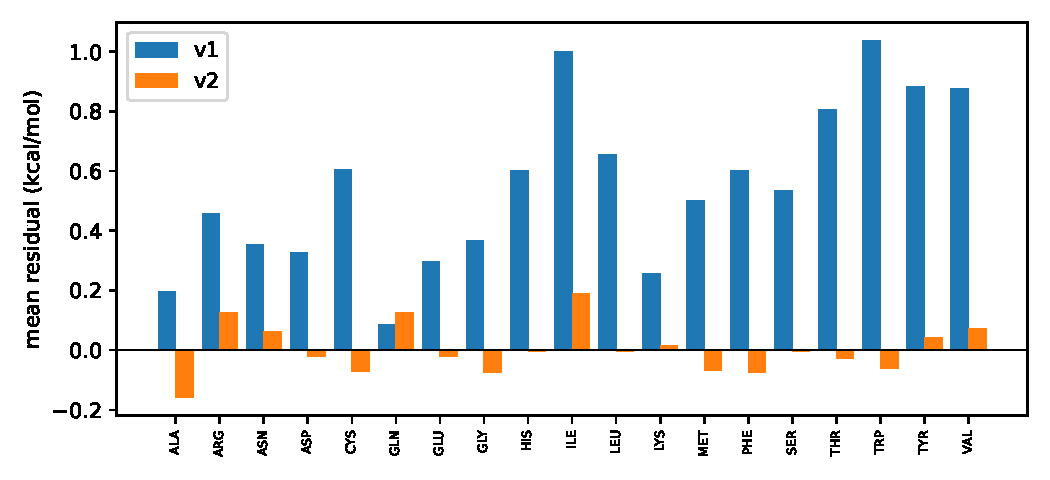
\includegraphics[width=0.9\textwidth]{figs/fig2_identity_bias.pdf}
\caption{Per-mutant-identity mean residual (predicted $-$ experimental)
on S2648 for the v1 and v2 models.}
\label{fig:bias}
\end{figure}

\subsection{p53 generalization and validation-based selection}
\label{sec:val}
A 15\% PDB-grouped validation split of S2648 (no structure shared with
training) was used to study checkpoint selection without touching the
test sets. Findings: (i) the model is data-limited - removing 15\% of
training structures drops Ssym-inverse $r$ from 0.578 to 0.434;
(ii) validation-$r$ peaks at epoch 5 ($r=0.400$) and then declines while
test $r$ keeps rising, so validation-based early stopping selects a
strictly worse checkpoint here (epoch-5 model: Ssym-inv $r=0.326$);
(iii) p53 remains out-of-family for the full-data model
($r=0.155$, vs v1's 0.451). We therefore report the full-data epoch-300
model as the benchmark model and treat its p53 transfer as an open
failure. Figure~\ref{fig:curve} shows the training/validation curves.

\begin{figure}[ht]
\centering
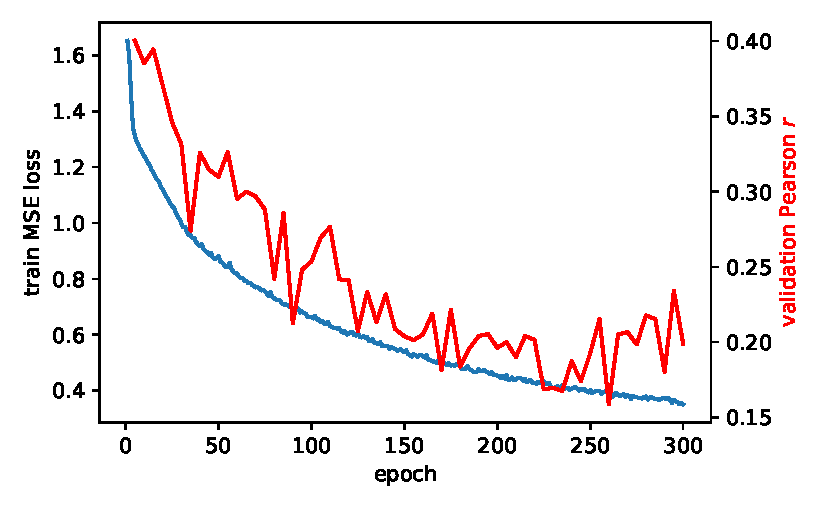
\includegraphics[width=0.7\textwidth]{figs/fig3_training_curve.pdf}
\caption{Training loss and grouped-validation Pearson $r$ over 300
epochs (validation run).}
\label{fig:curve}
\end{figure}

\subsection{Rescue scan on p53-Y220C (2VUK)}
\label{sec:scan}
All 3743 single substitutions of 2VUK chain A (197 positions $\times$
19) were scored with the v2 model and ranked raw and
identity-bias-corrected. Two structural facts frame the scan. First,
2VUK is Y220C crystallized on the superstable M133L/V203A/N239Y/N268D
background \cite{joerger2006}, so the scan measures stabilization
\emph{beyond} the known quadruple mutant. Second, the scan exposed an
out-of-distribution failure: S2648 and Ssym contain no proline mutations
in either direction, so the proline feature channel is untrained and
WT=PRO predictions are inflated (mean $+3.42$ vs $-0.39$~kcal/mol for
other WT types). All candidate rankings mask the 285 WT=PRO rows.

Face-validity against curated literature suppressors: L137R, a
documented Y220C second-site suppressor, scores $+3.13$ (top 7.2\%) and
H178Y (a G245S suppressor) $+5.67$ (top 0.9\%); the four superstable
background mutations are already present in the structure. The second
documented Y220C suppressor, A138G, is scored $-3.25$ (bottom 7\%) - a
clear miss, preserved as such. Top novel candidates (H178C $+6.7$,
H178M $+6.2$, H178D $+6.2$, H179R $+5.8$, A189Y $+5.5$, K139V $+5.3$)
concentrate in the two loops that host the known suppressors
(L137/K139 and H178/H179), which is the strongest plausibility signal
in the scan. Predicted magnitudes exceed typical experimental
stabilizations, and a greedy multi-mutant sum ($+42.6$~kcal/mol) is
implausible; ranks, not absolute values, are the output.

\subsection{SOD1 (Study 2)}
\label{sec:sod1}
Validation against 8 unique ThermoMutDB SOD1 $\Delta\Delta G$
measurements (duplicates across temperatures averaged; structures
1SPD/3ECU/1N18) gives Pearson $r=-0.05$, Spearman $-0.14$, MAE
2.66~kcal/mol, sign accuracy 25\%: the model does not generalize to
SOD1. The two worst misses have mechanistic explanations outside the
model class: A4V (exp $-7.2$, pred $+0.07$) was measured on metal-free
apo SOD1, and C6A ($-3.03$ vs $+0.1$) acts by removing an
aggregation-prone free cysteine - intermolecular disulfide chemistry
invisible to a single-chain contact graph. A whole-chain scan of WT SOD1
(1SPD) nominates V5Y/V5R and G114F/G114C as stabilizing candidates;
C111S, the one free-cysteine removal the model could in principle see,
ranks top 26\% with the correct sign. These are hypotheses with explicit
caveats, not claims.

\section{Limitations and negative results}
\label{sec:limits}
All of the following are preserved with quantification in
\texttt{results/}: (1) v1 aromatic-identity bias ($+0.76$ to
$+0.99$~kcal/mol); (2) greedy multi-mutant sums are implausible under
the independence approximation ($+17.5$ v1, $+42.6$ v2); (3) p53
transfer collapses at long training ($r$ 0.451 v1 $\to$ 0.155 v2-e300)
and validation-based early stopping does not repair it; (4) proline
positions are out of distribution because the training data contain no
proline mutations; (5) SOD1 $\Delta\Delta G$ prediction fails outright
($r=-0.05$, $n=8$); (6) the documented Y220C suppressor A138G is missed;
(7) scan magnitudes are inflated and only ranks should be read.

\section{External tools}
\label{sec:tools}
Tools actually executed or queried (honest ledger:
\texttt{results/EXTERNAL\_TOOLS.md}): RCSB PDB (484 structures),
ProtDDG-Bench, the Pucci 2018 published Table~1 (verified from PDF),
FireProtDB 2.0 REST API, ThermoMutDB API, Europe PMC REST, Zenodo API,
SoDCoD, NumPy (all model math), matplotlib (figures), pytest (24
hermetic tests), git/GitHub, Google Drive, pdflatex (this document).
Staged and planned entries are listed separately in the ledger and are
not counted here.


\begin{thebibliography}{9}
\bibitem[Pucci et al.(2018)]{pucci2018} Pucci F, Schwersensky M, Rooman M.
Artificial neural network applied to stability prediction of mutations.
\textit{Bioinformatics} 34:i367--i374 (2018). doi:10.1093/bioinformatics/bty348.
\bibitem[Pucci et al.(2016)]{pucci2016} Pucci F, Rooman M.
Physical and molecular bases of protein thermal stability and cold adaptation.
\textit{Curr Opin Struct Biol} 42:117--128 (2017).
\bibitem[Lindberg et al.(2005)]{lindberg2005} Lindberg MJ, Bystr\"om R,
Bokn\"as N, Andersen PM, Oliveberg M. Systematically perturbed folding
patterns of ALS-associated SOD1 mutants. \textit{PNAS} 102:9754--9759 (2005).
\bibitem[Joerger et al.(2006)]{joerger2006} Joerger AC, Ang HC, Fersht AR.
Structural basis for understanding oncogenic p53 mutations and designing
rescue drugs. \textit{PNAS} 103:15056--15061 (2006).
\end{thebibliography}
\end{document}
